\providecommand{\main}{..}
\documentclass[\main/main.tex]{subfiles}

\begin{document}
\graphicspath{{img/}{03_firmware/img/}}

\chapter{Ranging system architecture}
This section provides a detailed description of the ranging network operation and layered system architecture.

\section{Prerequisite}
Before getting into, we should cover some fundamental definitions. It will make it easier for further discussions. 

\subsection{Host and device}
The implemented UWB ranging system consists of one host and one device.
\begin{itemize}
    \item Host: the MCU which control the radio IC 
    \item Device: the radio IC transmitting and receiving over-the-air packet
\end{itemize}

\begin{figure}[H]
    \begin{center}
        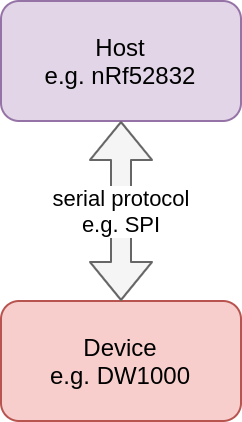
\includegraphics[scale=0.3]{host_device.png}
    \end{center}
    \caption{Host-device}
    \label{fig:host_device}
\end{figure}

\subsection{Timing system}
\label{subsec:timing_system_subsection}
Since there are two running systems: \textbf{host} and \textbf{device}, there are two timing systems. Unfortunately, these two timing systems do not have an agreement in the smallest unit of time. A host can use a $1\mu s$ -resolution timer due to the number of redundancy timers it has. A device, on the other hand, may not have as many timers and clock source as a host has, so the device timing system is limited. In the case of DW1000 radio IC, $1\mu s$ is approximately 512 counts of the fundamental 499.2 MHz UWB clock which is actually \textbf{$\sim 1.026\mu s$}. 

For precise timing, the implementation does not make any assumption about the equality of $1\mu s$ in host and device. Timestamp in the device must be converted to host reference for further processing, upon completion, the result must be converted back to the device reference before writing to that device. 
\subsection{RMarker}
Because of the limited transmission speed, the interval between the begin of preamble and the end of PHY data unit is relatively large compared with the propagation interval. For the ultimate purpose of ranging using time of flight, a point should be considered to be marker for timestamping packet. As defined in the context of the IEEE 802.15.4-2015 standard \cite{IEEE_Std_802_15_4_2015}, RMarker is the first chip after the SFD, it also means that: RMarker defines the start of the PHR in either transmitter or receiver. 

\begin{figure}[H]
    \begin{center}
        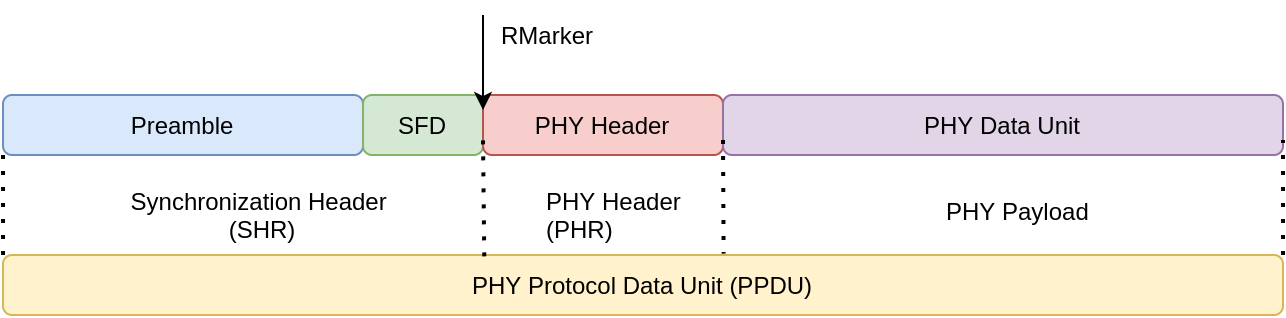
\includegraphics[scale=0.3]{802_15_4_physical.png}
    \end{center}
    \caption{802.15.4 RMarker}
    \label{fig:802_15_4_rmarker}
\end{figure}

\section{Layered architecture}
The ranging system is implemented follow 3 layers model as shown in figure \ref{fig:ranging_layered_architecture}. 
\begin{itemize}
    \item CCP (Clock Calibration Packet) provides synchronization service for the upper layer. All nodes jointed to the network will be synced each time a new superframe start.
    \item TDMA (Time Division Multiple Access): Each superframe is divided into multiple slots. TDMA layer provides slot service for its upper layer. 
    \item TWR (Two Way Ranging) layer runs ranging session in the time slot provided by TDMA layer.
\end{itemize}

Follow the bottom-up approach, detail description about each layer is provided in following sections.
\begin{figure}[H]
    \begin{center}
        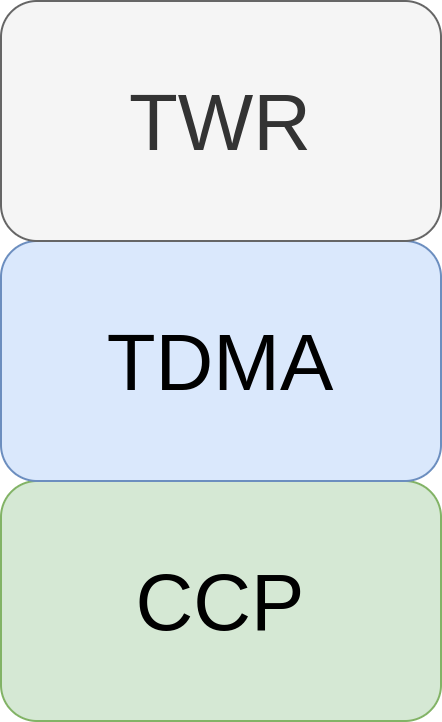
\includegraphics[scale=0.3]{ranging_layered_architecture}
    \end{center}
    \caption{Ranging layered architecture}
    \label{fig:ranging_layered_architecture}
\end{figure}

\section{Clock calibration packet (CCP)}
The main role clock calibration packet is to provide the superframe synchronization between nodes. 
\subsection{CCP role}
Three CCP roles are defined, allowing nodes to sync with others: Master, Slave, Relay.
\begin{itemize}
    \item \textbf{CCP master}: There is only and only one master node over the network. The master node is the only place where a clock calibration packet is produced. It will produce and transmit the clock calibration packet with the interval defined as a constant in the firmware. My implementation use the value of 100ms for such interval. 
    \item \textbf{CCP slave}: Slave nodes listen for the clock calibration packet to start their internal timer for each superframe.
    \item \textbf{CCP relay}: Relay nodes repeat the clock calibration packet to extend the network physical area. Before repeating the packets, they must do some modification so the receiver can sync with the  master node. There is a constraint in the maximum of repeat level which will be analyzed afterward.
\end{itemize}

To initialize the system, at least one of many nodes must be chosen as a master. The master node will start and control the network and allow other nodes to join and form a network. It is possible to configure more than one node as master, but only one will be active and the others will take the role of slave and/or replay node. A node can take the slave and relay roles at the same time.

\subsection{CCP frame format}
The ccp frame used for synchronization shall be formatted as illustrated in figure \ref{fig:ccp_blink_frame}. The format follow the IEEE 802.15.4-2015 \cite{IEEE_Std_802_15_4_2015} multipurpose frame.
\begin{figure}[H]
    \centering
    \begin{bytefield}[bitwidth=1.1em]{32}
        \bitheader{0-31} \\
        \begin{rightwordgroup}{IEEE \\ header}
            \bitbox{8}{frame control} & 
            \bitbox{8}{sequence number} & \\ 
            \bitbox{32}{extended unique identifier high} \\ 
            \bitbox{32}{extended unique identifier low}
        \end{rightwordgroup} \\
        \begin{rightwordgroup}{Custom\\payload}
            \bitbox{16}{short address} &
            \bitbox{16}{transmission interval high} \\
            \bitbox{32}{transmission interval low} \\
            \bitbox{32}{transmission timestamp high} \\ 
            \bitbox{32}{transmission timestamp low}\\
            \bitbox{8}{repeat count} &
            \bitbox{8}{repeat max}
            \bitbox{16}{epoch to rm us}
        \end{rightwordgroup}
    \end{bytefield}
    \caption{CCP blink frame}
    \label{fig:ccp_blink_frame}
\end{figure}

\subsubsection{Frame Control}
The Frame Control field for the Multipurpose frame are specified in figure \ref{fig:multipurpose_frame_control_field}. Follow standard described in section 7.3.5 of IEEE 802.15.4 \cite{IEEE_Std_802_15_4_2015}, the field is filled up for the purpose of synchronization frame.

\begin{figure}[H]
    \centering
    \begin{bytefield}[bitwidth=6em, bitheight=3em]{8}
        \bitheader{0-7} \\
        \bitbox{3}{Frame Type} &
        \bitbox{1}{Long Frame Control} &
        \bitbox{2}{Destination Addressing Mode} &
        \bitbox{2}{Source Addressing Mode}
        % \bitbox{1}{PAN ID Present} &
        % \bitbox{1}{Security Enabled} &
        % \bitbox{1}{Sequence Number Suppression} &
        % \bitbox{1}{Frame Pending} &
        % \bitbox{2}{Frame Version} &
        % \bitbox{1}{Ack Request} &
        % \bitbox{1}{IE Present}
    \end{bytefield} 
    \caption{Multipurpose frame control field}
    \label{fig:multipurpose_frame_control_field}
\end{figure}
The Frame Type field shall contain the value that indicates a Multipurpose frame as define in IEEE 802.15.4-2015 ($b_2 b_1 b_0 = 101$).

The Long Frame Control field shall be set to \textbf{0} to indicate an MP Short Frame Control field (only bits 0 to 7 make up the Frame Type field).

The Destination Addressing Mode field shall be set to \textbf{0} to indicate PAN ID and destination address fields are not present.

The Source Addressing Mode field shall be set to \textbf{11} to indicate source address field contains an extended address (64-bit Extended Unique Identifier).

For the synchronization purpose, the final value of this field is \textbf{0xC5}.

\subsubsection{Sequence Number}
The Sequence Number field specifies the sequence identifier for the frame.

\subsubsection{Extended Unique Identifier}
Extended Unique Identifier as its name, it is 64-bit unique ID for each device over the globe. DW1000 radio IC takes it from its lot id and part id written by the manufacturer.

\begin{equation}
    \texttt{ euid = ((uint64\_t)lot\_id) << 32 + part\_id}
\end{equation}

\subsubsection{Short address}
The address of sending node in the TDMA network.
\begin{equation}
   \texttt{ short\_address = (uint16\_t)euid \& 0xFFFF}
\end{equation}

\subsubsection{Transmission Interval}
The interval of a superframe, unit of time is a microsecond of DW1000 timer. As previously discussed, 1 microsecond of DW1000 is approximately 512/499.2Mhz. The implementation uses the value of 0x20000, which mean that the transmission interval is:
\begin{equation}
    \texttt{0x20000*(512/499.2Mhz) = 127795.2$\mu$s = 127.7952ms}
\end{equation}

\subsubsection{Transmission Timestamp}
The moment that RMarker is transmitted is the event nominated as the transmit time-stamp. The DW1000 digital transmit circuitry takes note of the system clock counter as the RAW transmit timestamp at the point when it begins sending the PHR. It then adds to this the transmit antenna delay to get the antenna adjusted transmit timestamp.

\subsubsection{Repeat count}
It is the number of non-master nodes that the ccp packet traveled before coming to this node.

\subsubsection{Repeat max}
It is the maximum number of repetition times per packet of ccp.

\subsection{CCP master selection algorithm}

When designing a synchronous system, one of the most fundamental problems is the persistence of the synchronization source. Here, the question is: what will happen if the synchronization source fails, will it stop the entire system from working? This problem is known as the single point of failure (SPOF) problem. SPOFs are undesirable in any system with a goal of high availability or reliability.

To deal with SPOFs, in my implementation, there is no pre-configured node to be master. Instead, all nodes (except for the tag node) can be a master. So, how a node decides itself to be a master or slave? The main idea is the lazy mindset: master is hard work, I will not take it, but if nobody does, I will. Figure \ref{fig:CCP_state_diagram} illustrates this mindset.

\begin{figure}[H]
    \begin{center}
        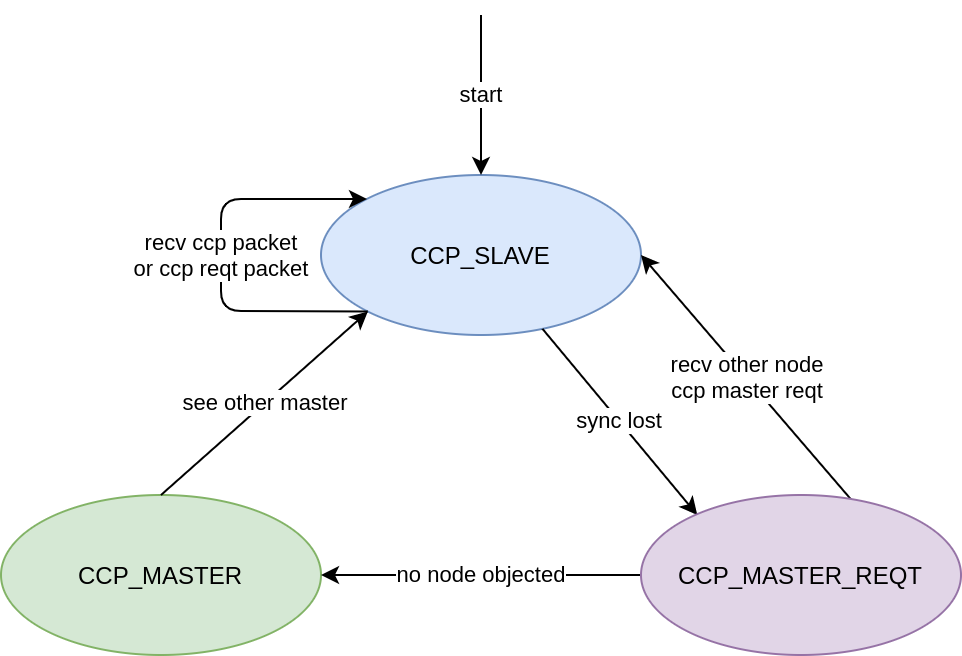
\includegraphics[scale=0.35]{ccp_state_diagram.png}
    \end{center}
    \caption{CCP state transition diagram}
    \label{fig:CCP_state_diagram}
\end{figure}

As shown in figure \ref{fig:CCP_state_diagram}, all node will start with ccp slave role. If there is already a master node, a just-powered-on node will receive ccp packets from the master node and remain in the slave state. If there is no master node, after its internal counter reaches a conditional random thresh hold, it will turn into the master request state. It now sends ccp request packets and listens for objection for a while. If no node object, the new state is ccp master. If it receives any ccp packet or ccp request packet in the master or master request state, it will immediately turn into the slave state as it is lazy.

Figure \ref{fig:ccp_slave_flow_chart}, \ref{fig:ccp_master_reqt_flow_chart} and \ref{fig:ccp_master_flow_chart} are simplified flowcharts used for implementing each state.

Figure \ref{fig:ccp_slave_flow_chart} is the flow chart for CCP\_SLAVE state. In this state, rx\_timeout\_counter variable is used to timeout the slave and turn it into the CCP\_MASTER\_REQT state.
This variable is also checked for each RX timer callback, if it is not equal to 0, which means that there is a timeout event before, it is necessary to listen immediately to increase the chance of receiving the next ccp packet. If the variable equal to 0, the MCU will schedule the radio IC to receive the frame at a calculated moment. If a ccp packet is successfully received, MCU will schedule the next wake up to receive the next ccp packet based on the ccp packet it just received. 

\begin{figure}[H]
    \begin{center}
        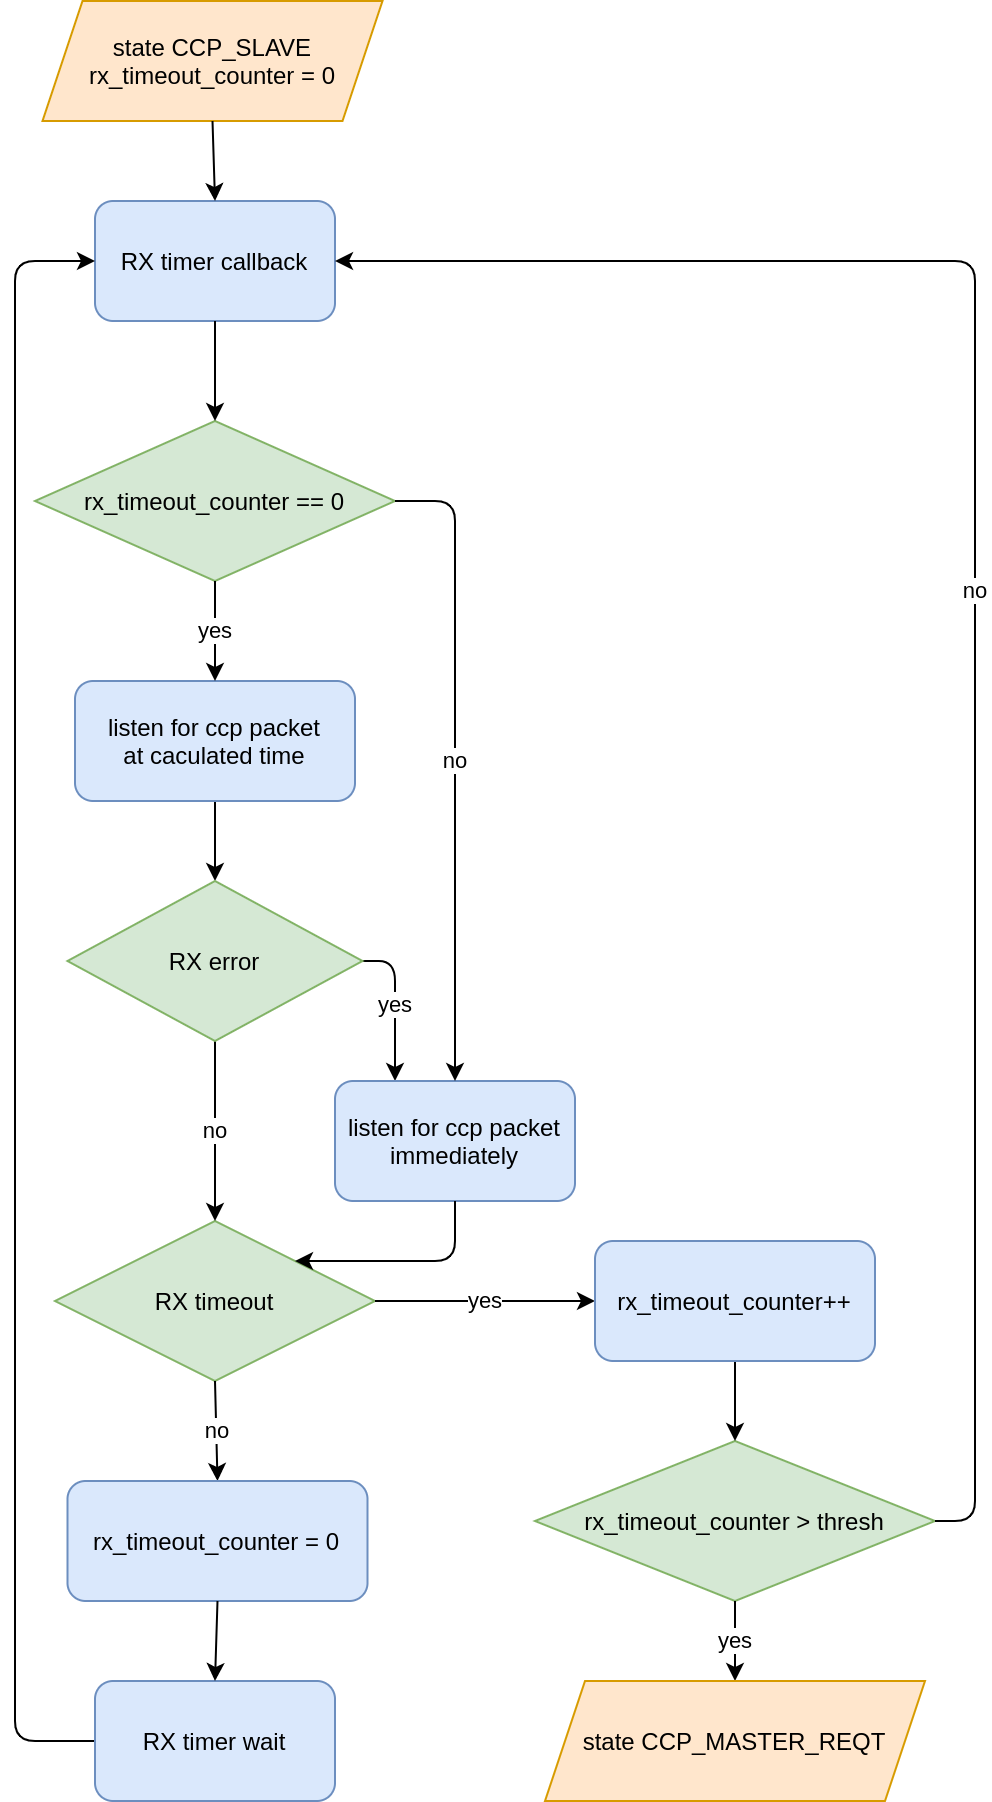
\includegraphics[scale=0.35]{ccp_slave_flow_chart.png}
    \end{center}
    \caption{CCP slave flow chart}
    \label{fig:ccp_slave_flow_chart}
\end{figure}

Figure \ref{fig:ccp_master_reqt_flow_chart} is the flow chart for
CCP\_MASTER\_REQT state. In this state, a node will periodically send the ccp request packet. If no node protests by sending another cpp packet or ccp request packet, the variable master\_reqt\_state is used to timeout the CCP\_MASTER\_REQT state and turn the node into the master state.

Figure \ref{fig:ccp_master_flow_chart} is the flow chart for CCP\_MASTER state. A node enters this state by scheduling a TX timer and waiting for its timeout. This timer will wake up the CPU to schedule the radio IC for transmitting ccp packet at a calculated moment. The listen stage here is for the demonstration purpose only. In fact, the ccp packet does not listen in the master state. Instead, the ccp implementation act as an observer to analyze any packet received in the superframe internal interval. Packets must be received by listen commands of higher layers.

\begin{figure}[H]
    \begin{center}
        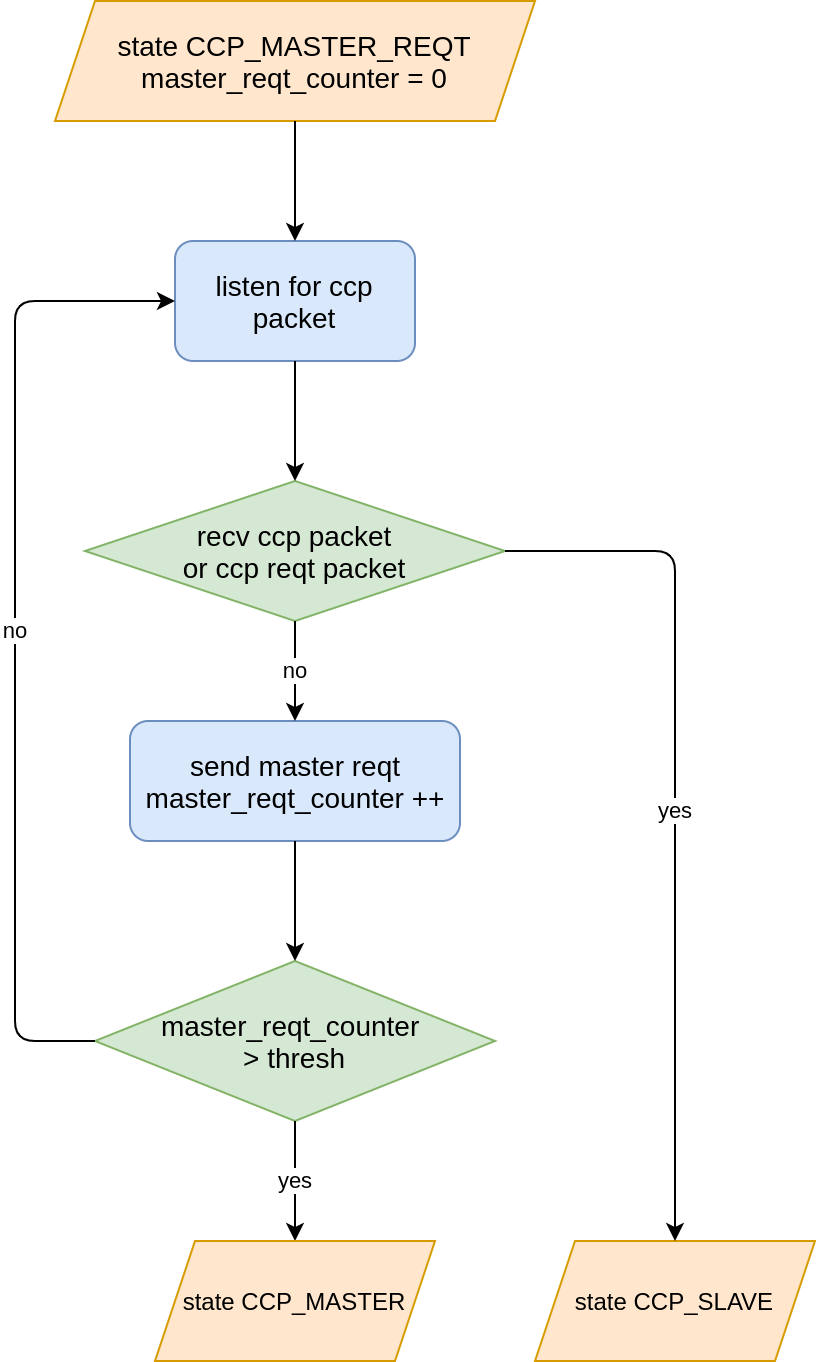
\includegraphics[scale=0.35]{ccp_master_reqt_flow_chart.png}
    \end{center}
    \caption{CCP master request flow chart}
    \label{fig:ccp_master_reqt_flow_chart}
\end{figure}


\begin{figure}[H]
    \begin{center}
        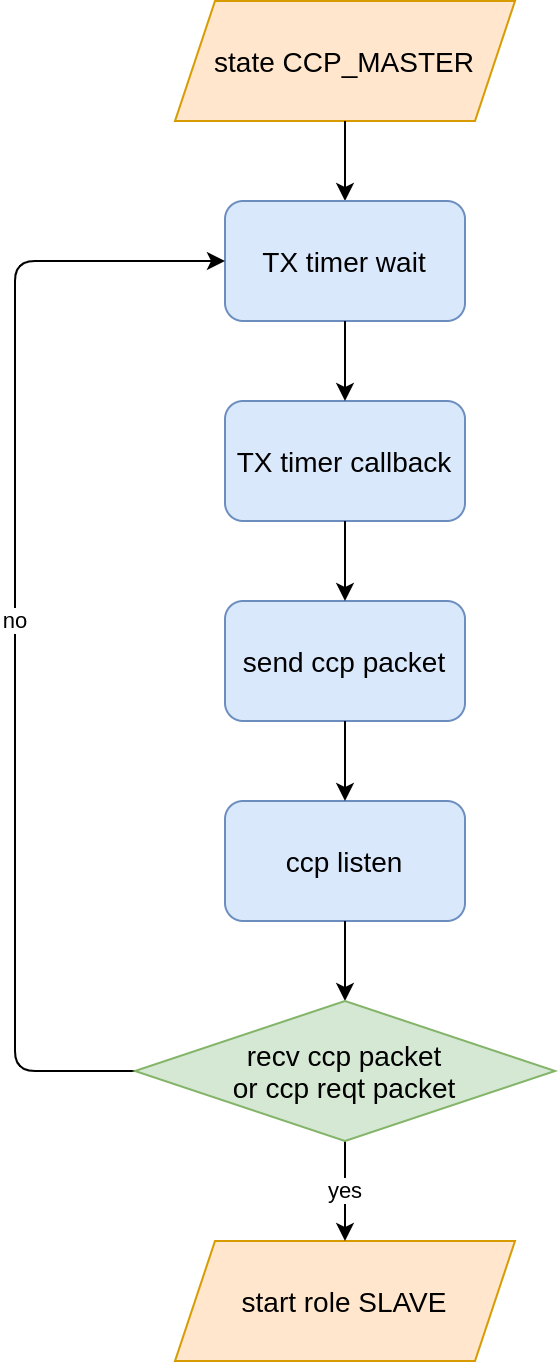
\includegraphics[scale=0.35]{ccp_master_flow_chart.png}
    \end{center}
    \caption{CCP master flow chart}
    \label{fig:ccp_master_flow_chart}
\end{figure}

% \begin{figure}
%     \begin{subfigure}[b]{0.45\textwidth}
%         \begin{center}
%         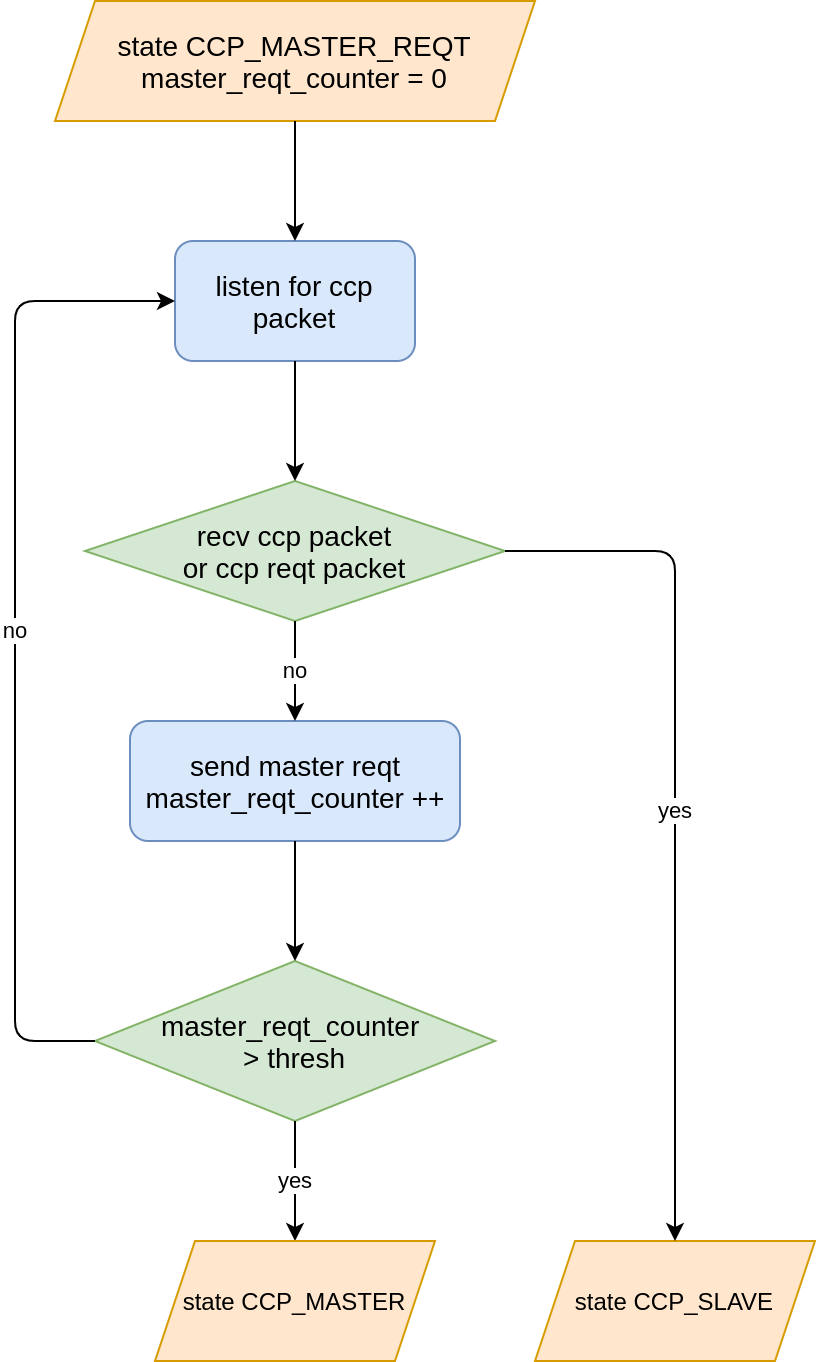
\includegraphics[scale=0.25]{ccp_master_reqt_flow_chart.png}
%     \end{center}
%         \caption{CCP master request flow chart}
%         \label{fig:ccp_master_reqt_flow_chart}
%     \end{subfigure}
%     %
%     \begin{subfigure}[b]{0.45\textwidth}
%         \begin{center}
%     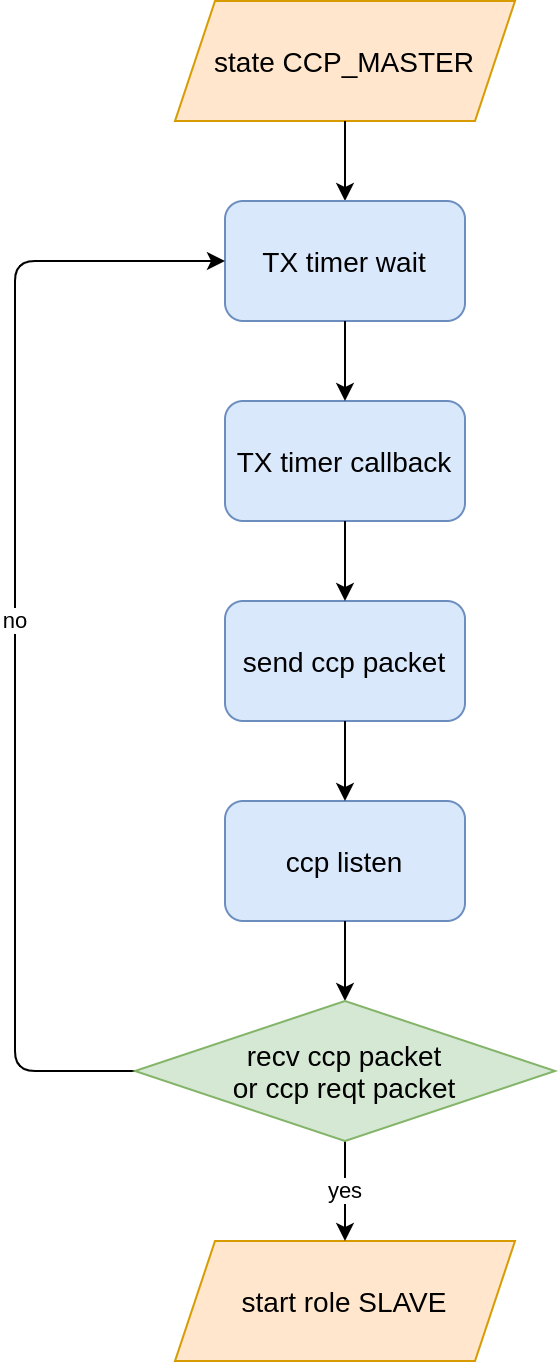
\includegraphics[scale=0.3]{ccp_master_flow_chart.png}
% \end{center}
%     \caption{CCP master flow chart}
%     \label{fig:ccp_master_flow_chart}
%     \end{subfigure}
%   \end{figure}

\subsection{CCP implementation}
This section discusses detailed timing problems related to CCP. Before starting, some fundamental concepts should be defined and accepted:
\begin{itemize}
    \item Master epoch $ep_m$: Packet timestamp referenced to CCP master device timing system.
    \item Local epoch $ep_l$: Packet timestamp referenced to CCP slave device timing system.
    \item Os epoch $ep_o$: Packet timestamp referenced to CCP master or slave host timing system.
    \item Period $\tau$: The interval of a superframe.
    \item $T_{er}$: The interval between an epoch and a RMarker as shown in figure \ref{fig:ccp_epoch_and_rmarker}.
    \item $t_k$: Timestamp for $k$th frame in device timing system.
    \item $t_h$: Current host time (in host timing system).
    \item $t_d$: Current device time (in device timing system).
    \item $f_{d2h}$: A linear function for converting the device time to host time as explained in \ref{subsec:timing_system_subsection}
    \item $T_{latency}$: OS latency is the interval for OS to process before sending.
\end{itemize}
\begin{figure}[H]
    \begin{center}
        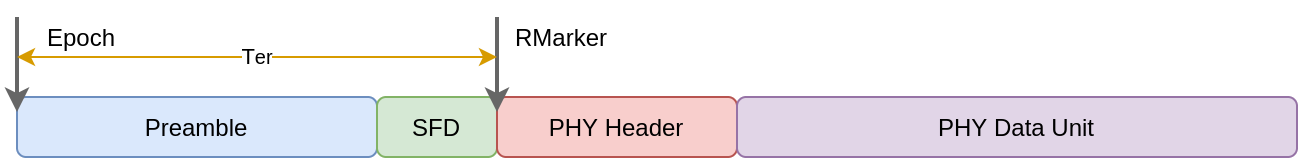
\includegraphics[scale=0.35]{ccp_epoch_and_rmarker.png}
    \end{center}
    \caption{CCP epoch and RMarker}
    \label{fig:ccp_epoch_and_rmarker}
\end{figure}

\subsubsection{CCP timing for master node}

The CCP packet is sent with timestamp calculated from previous frame:
\begin{equation}
    t_k = t_{k-1} + \tau
\end{equation}

Each time the CCP master node complete to send a CCP packet, a TX event is called for re-calculating $ep_m$, $ep_l$ and $ep_o$ using the following formulas.
\begin{equation}
    ep_m = ep_l = t_k - T_{er}
\end{equation}

\begin{equation}
    ep_o = t_h - f_{d2h}(t_d - t_k) - T_{er}
\end{equation}

After sending the CCP packet, the MCU will schedule for the next wake up at:
\begin{equation}
    t_{wake up} = ep_o + \tau - T_{latency}
\end{equation}

\begin{figure}[H]
    \begin{center}
        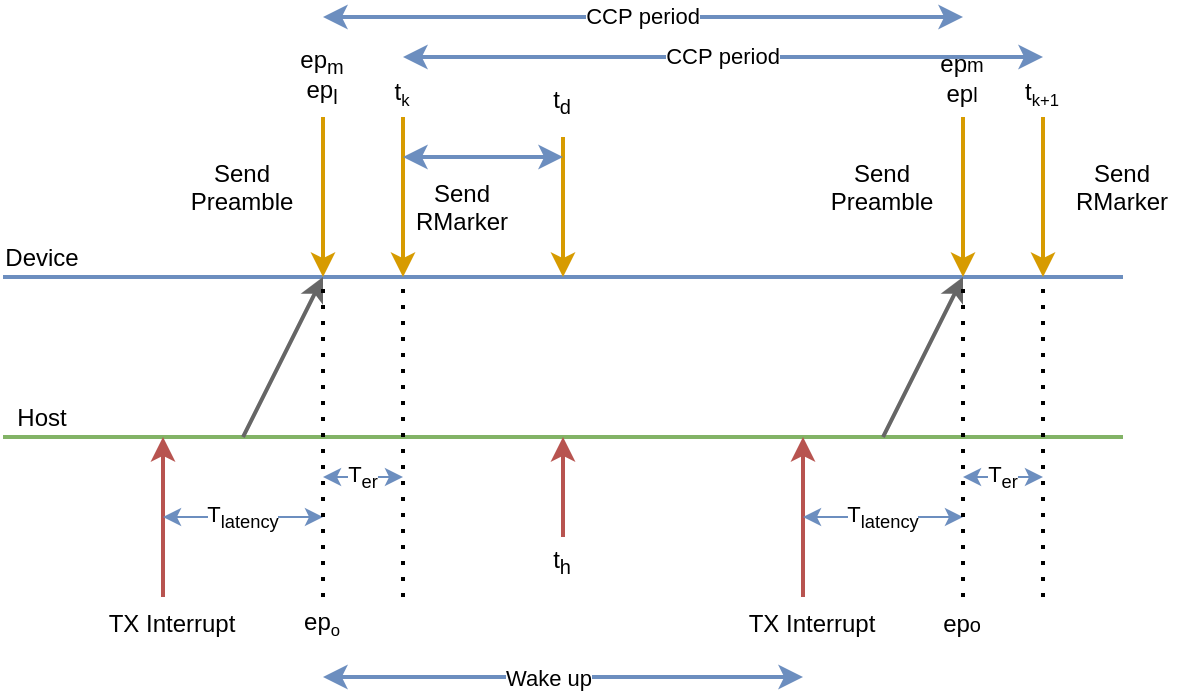
\includegraphics[scale=0.30]{ccp_timing_for_master_node.png}
    \end{center}
    \caption{CCP master timing}
    \label{fig:interupt_latency_master}
\end{figure}

\subsubsection{CCP calculation for slave node}
\begin{figure}[H]
    \begin{center}
        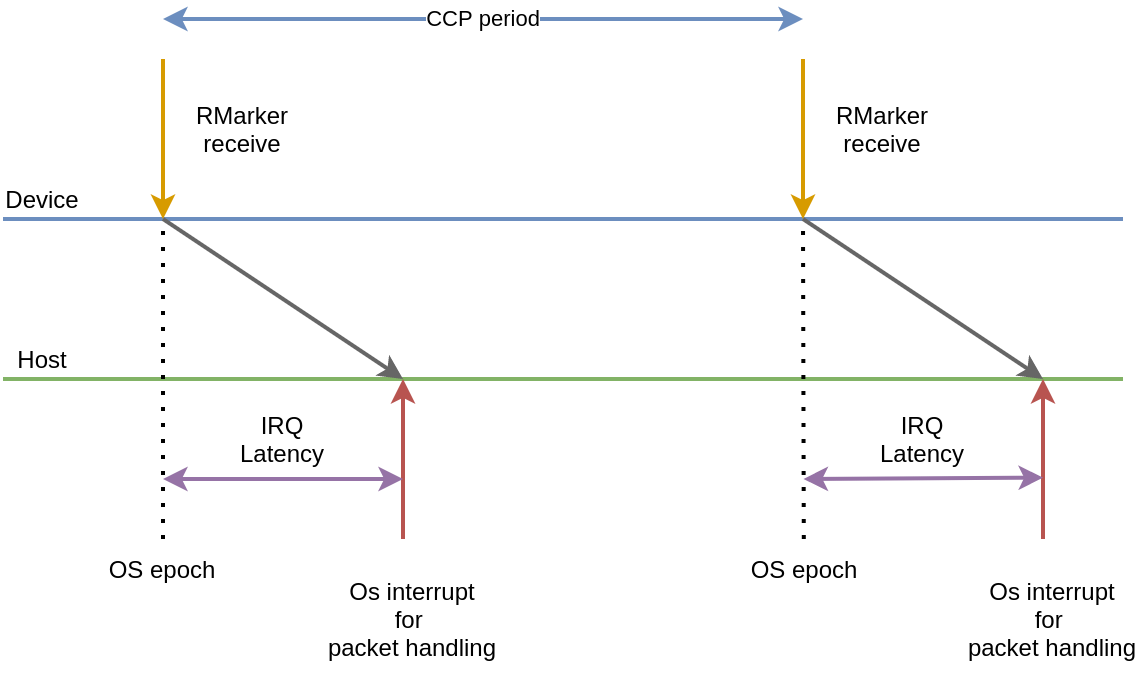
\includegraphics[scale=0.35]{interupt_latency_listener.png}
    \end{center}
    \caption{interrupt latency listener}
    \label{fig:interupt_latency_listener}
\end{figure}

\subsubsection{Repeat CCP packet}
\begin{figure}[H]
    \begin{center}
        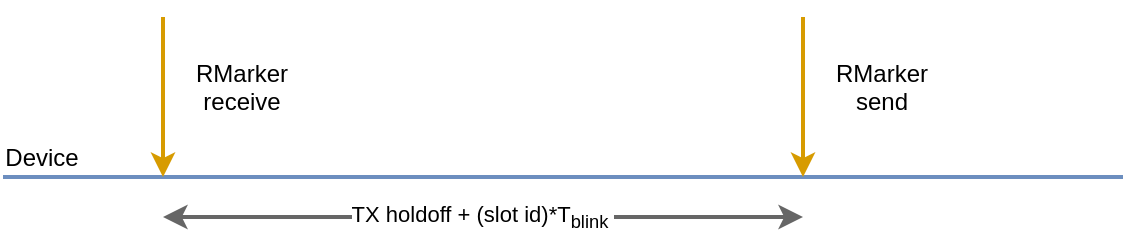
\includegraphics[scale=0.35]{ccp_repeat.png}
    \end{center}
    \caption{CCP Repeat}
    \label{fig:ccp_repeat}
\end{figure}


\section{Time Division Multiple Access (TDMA)}
The fundamental role of the TDMA layer is to give a notification to its upper layer when it is the time to run the service. To archive this, a node must firstly ask for getting an appropriate and available slot from jointed nodes.

\subsection{TDMA role}
In the TDMA layer, a jointed node must take one of two roles: Anchor or Tag.
\begin{itemize}
    \item TDMA Anchor: A node taking the role as an anchor must be fixed and broadcast its pre-configured location information to others.
    \item TDMA Tag: TDMA tag node is the mobile node needed to be located in the coordinate of anchors.
\end{itemize}

\subsection{TDMA slot}
The superframe is divided into multiple slots as shown in figure \ref{fig:tdma_slot}.
\begin{figure}[H]
    \begin{center}
        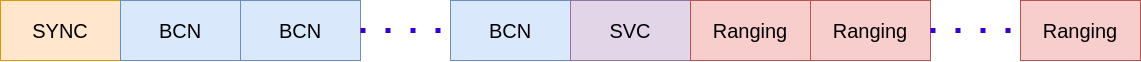
\includegraphics[scale=0.4]{tdma_slot.png}
    \end{center}
    \caption{TDMA slot}
    \label{fig:tdma_slot}
\end{figure}

\subsubsection{Synchronization slot (SYNC slot)}
In the SYNC slot interval, a master node produces and transmits the clock calibration packet. Relay nodes also repeat the clock calibration packet in this interval too.
\subsubsection{Beacon slot (BCN slot)}
An anchor node will broadcast its location and slot map information in its BCN slot. It is allowed for a jointed anchor to skip some superframes as long as it does not exceed a certain value. Other anchor nodes consider a node has left the network when they do not see any BCN message from such node for a number of superframes. The implementation uses the value of 10 for this purpose.
\subsubsection{SVC slot}
When a node wants to joint the network as a tag or anchor, it has to send its joint request in an SVC slot. The request is broadcasted and responded by all jointed anchors in their next assigned BCN slot.
\subsubsection{Ranging slot}
A jointed tag initiates the range request in its assigned ranging slot. During the remaining interval, it also listens for the response from anchors to calculate to ToF (Time of Flight).

\subsection{TDMA packet format}
The message include two parts: IEEE frame header and payload:
\begin{itemize}
    \item IEEE fame header conforms the 802.15.4-2016 standard
    \item Payload field may contain more than one message. Each message have TLV (type-length-value) format as shown in figure \ref{fig:tdma_frame_payload}. Currently, three message types are defined: \textbf{Slot request/response}, \textbf{Location}, \textbf{Slot map}. The value of these message type are illustrated in figure \ref{fig:slot_request_response_message}, \ref{fig:location_value}, \ref{fig:slot_map_message}.
\end{itemize}
\begin{figure}[H]
    \centering
    \begin{bytefield}[bitwidth=1.1em]{32}
        \bitheader{0-31} \\
        \begin{rightwordgroup}{IEEE \\ frame \\ header}
            \bitbox{16}{fctrl} & 
            \bitbox{8}{seq num} & \\ 
            \bitbox{16}{PANID} \\ 
            \bitbox{16}{dst address} &
            \bitbox{16}{src address}
        \end{rightwordgroup} \\
        \wordbox[tlr]{1}{payload} \\
        \wordbox[blr]{1}{$\cdots$}
    \end{bytefield}
    \caption{TDMA frame}
    \label{fig:tdma_frame}
\end{figure}

\begin{figure}[ht]
    \centering
    \begin{bytefield}[bitwidth=1.1em]{32}
        \bitheader{0-15}\\
        \bitbox{8}{type} & 
        \bitbox{8}{len} & 
        \bitbox{16}{value}
    \end{bytefield}
    \caption{TDMA frame payload}
    \label{fig:tdma_frame_payload}
\end{figure}

\begin{figure}[H]
    \centering
    \begin{bytefield}[bitwidth=2em]{16}
        \bitheader{0-15} \\
        \bitbox{8}{slot} &
        \bitbox{8}{slot request/response}
    \end{bytefield}
    \caption{Slot request/response message}
    \label{fig:slot_request_response_message}
\end{figure}

\begin{figure}[H]
    \centering
    \begin{bytefield}[bitwidth=1.1em]{32}
        \bitheader{0-31} \\
        \bitbox{8}{slot} \\
        \bitbox{32}{location x} \\
        \bitbox{32}{location y} \\ 
        \bitbox{32}{location z}
    \end{bytefield}
    \caption{Location message value}
    \label{fig:location_value}
\end{figure}

\begin{figure}[H]
    \centering
    \begin{bytefield}[bitwidth=1.1em]{32}
        \bitheader{0-31} \\
        \bitbox{8}{slot} \\
        \bitbox{32}{slot map high} \\
        \bitbox{32}{slot map low}
    \end{bytefield}
    \caption{Slot map message}
    \label{fig:slot_map_message}
\end{figure}

\subsection{Network management algorithm}

\subsubsection{State diagram}
The TDMA state diagram is shown in figure \ref{fig:tdma_state_diagram}. 
The master node is the initiator of the network. It has to be an anchor and occupy BCN slot 1. Since there is no jointed node before, the master node does not need to ask others. Hence, after ccp layer provides first synchronization, all nodes begin with REQT state except for the master node. 

\begin{figure}[H]
    \begin{center}
        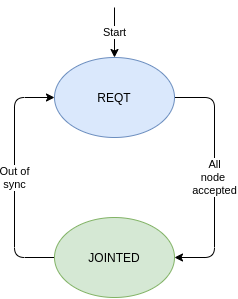
\includegraphics[scale=0.6]{tdma_state_diagram.png}
    \end{center}
    \caption{TDMA state diagram}
    \label{fig:tdma_state_diagram}
\end{figure}

\subsubsection{REQT state flow chart}
The REQT state implementation is illustrated in the follow chart \ref{fig:REQT_state_diagram}.
\begin{figure}[H]
    \begin{center}
        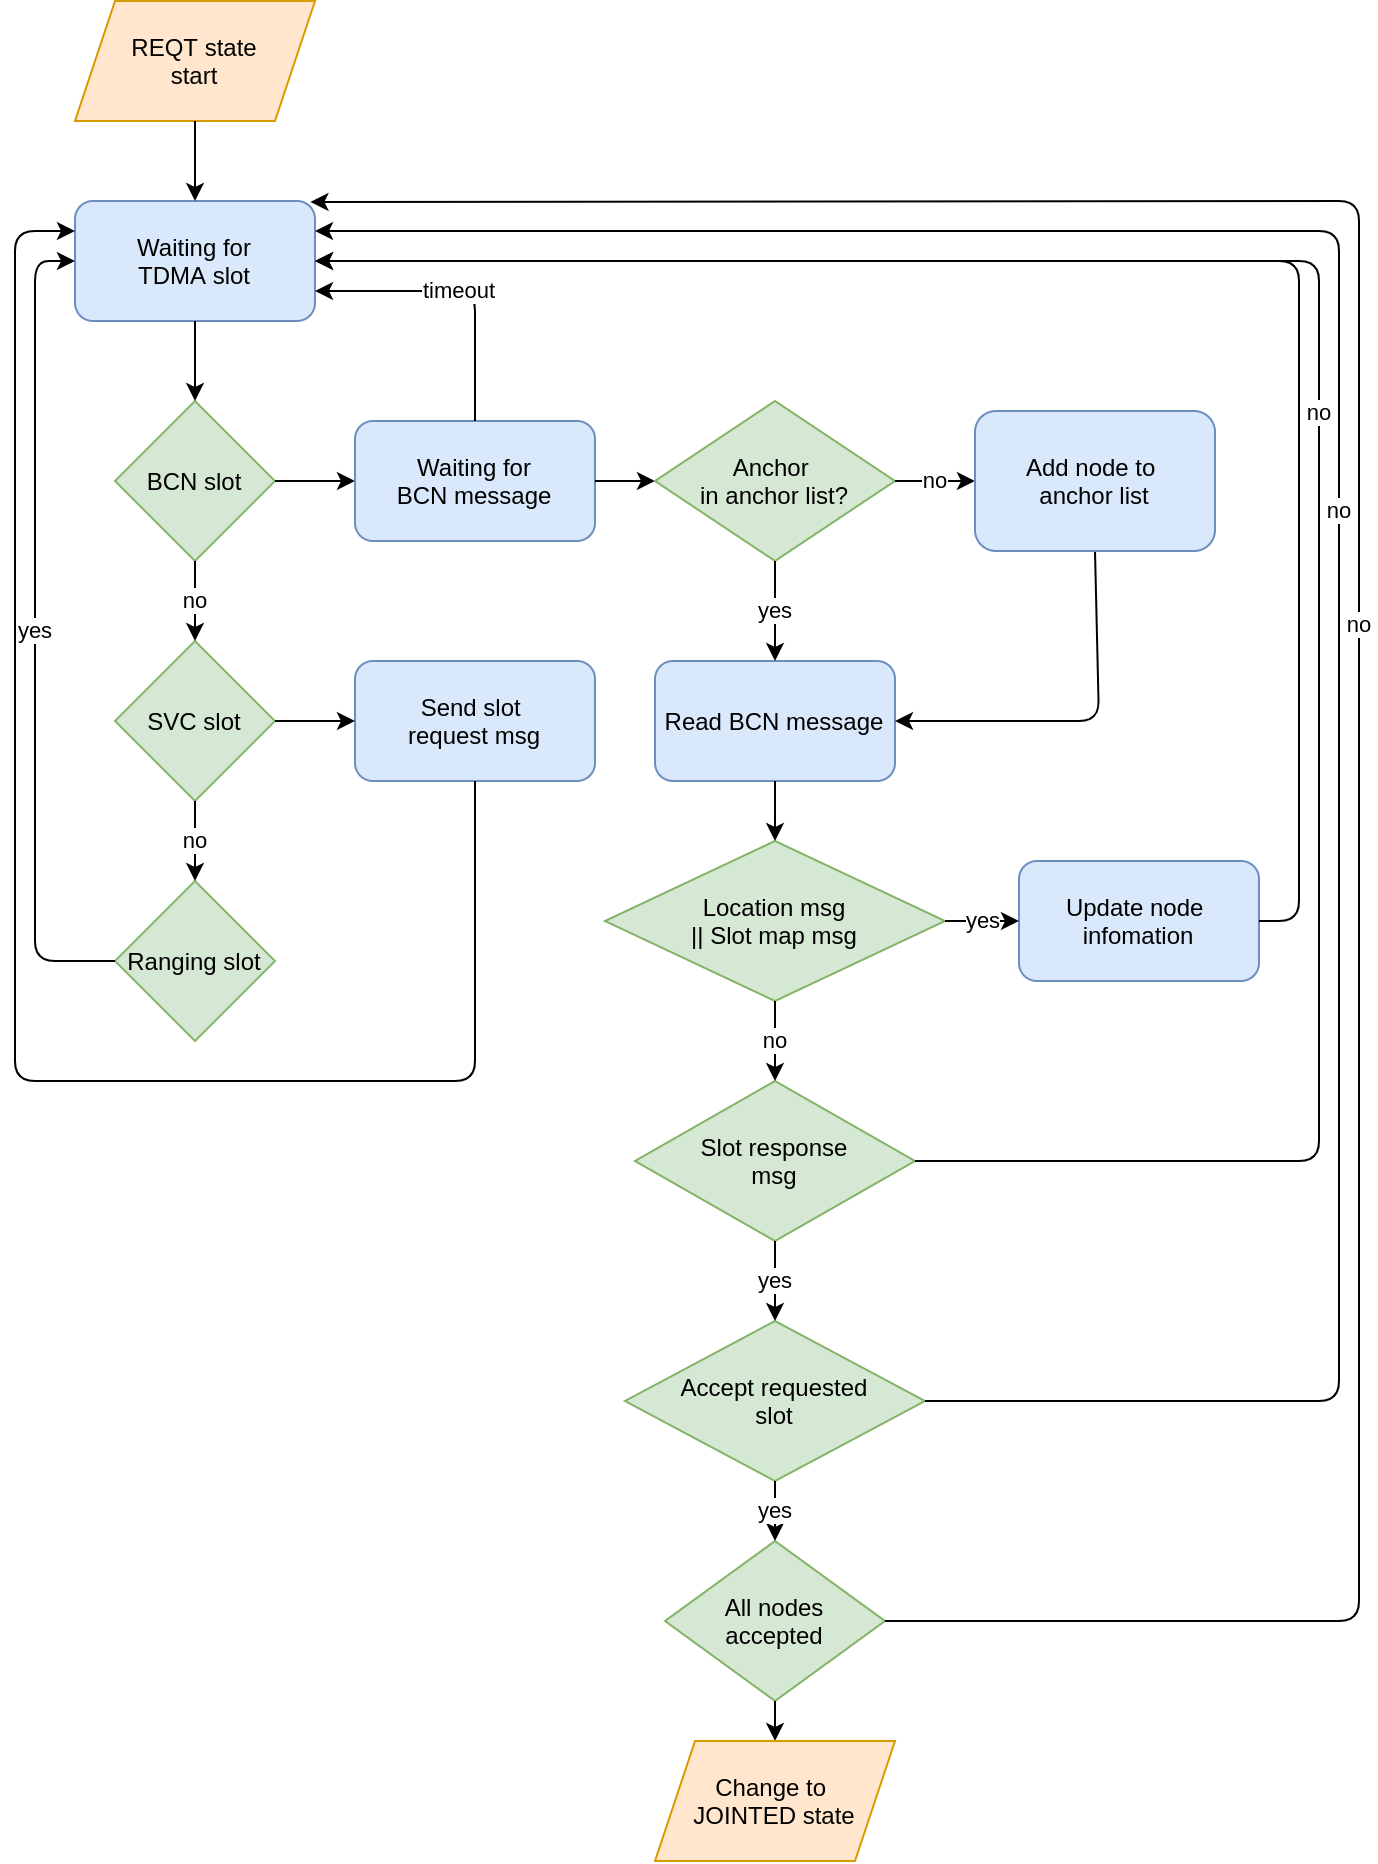
\includegraphics[scale=0.33]{REQT_flow_chart.png}
    \end{center}
    \caption{REQT state diagram}
    \label{fig:REQT_state_diagram}
\end{figure}

\subsubsection{JOINTED state flow chart}
The JOINTED state implementation is illustrated in the follow chart \ref{fig:JOINTED_state_diagram}
\begin{figure}[H]
    \begin{center}
        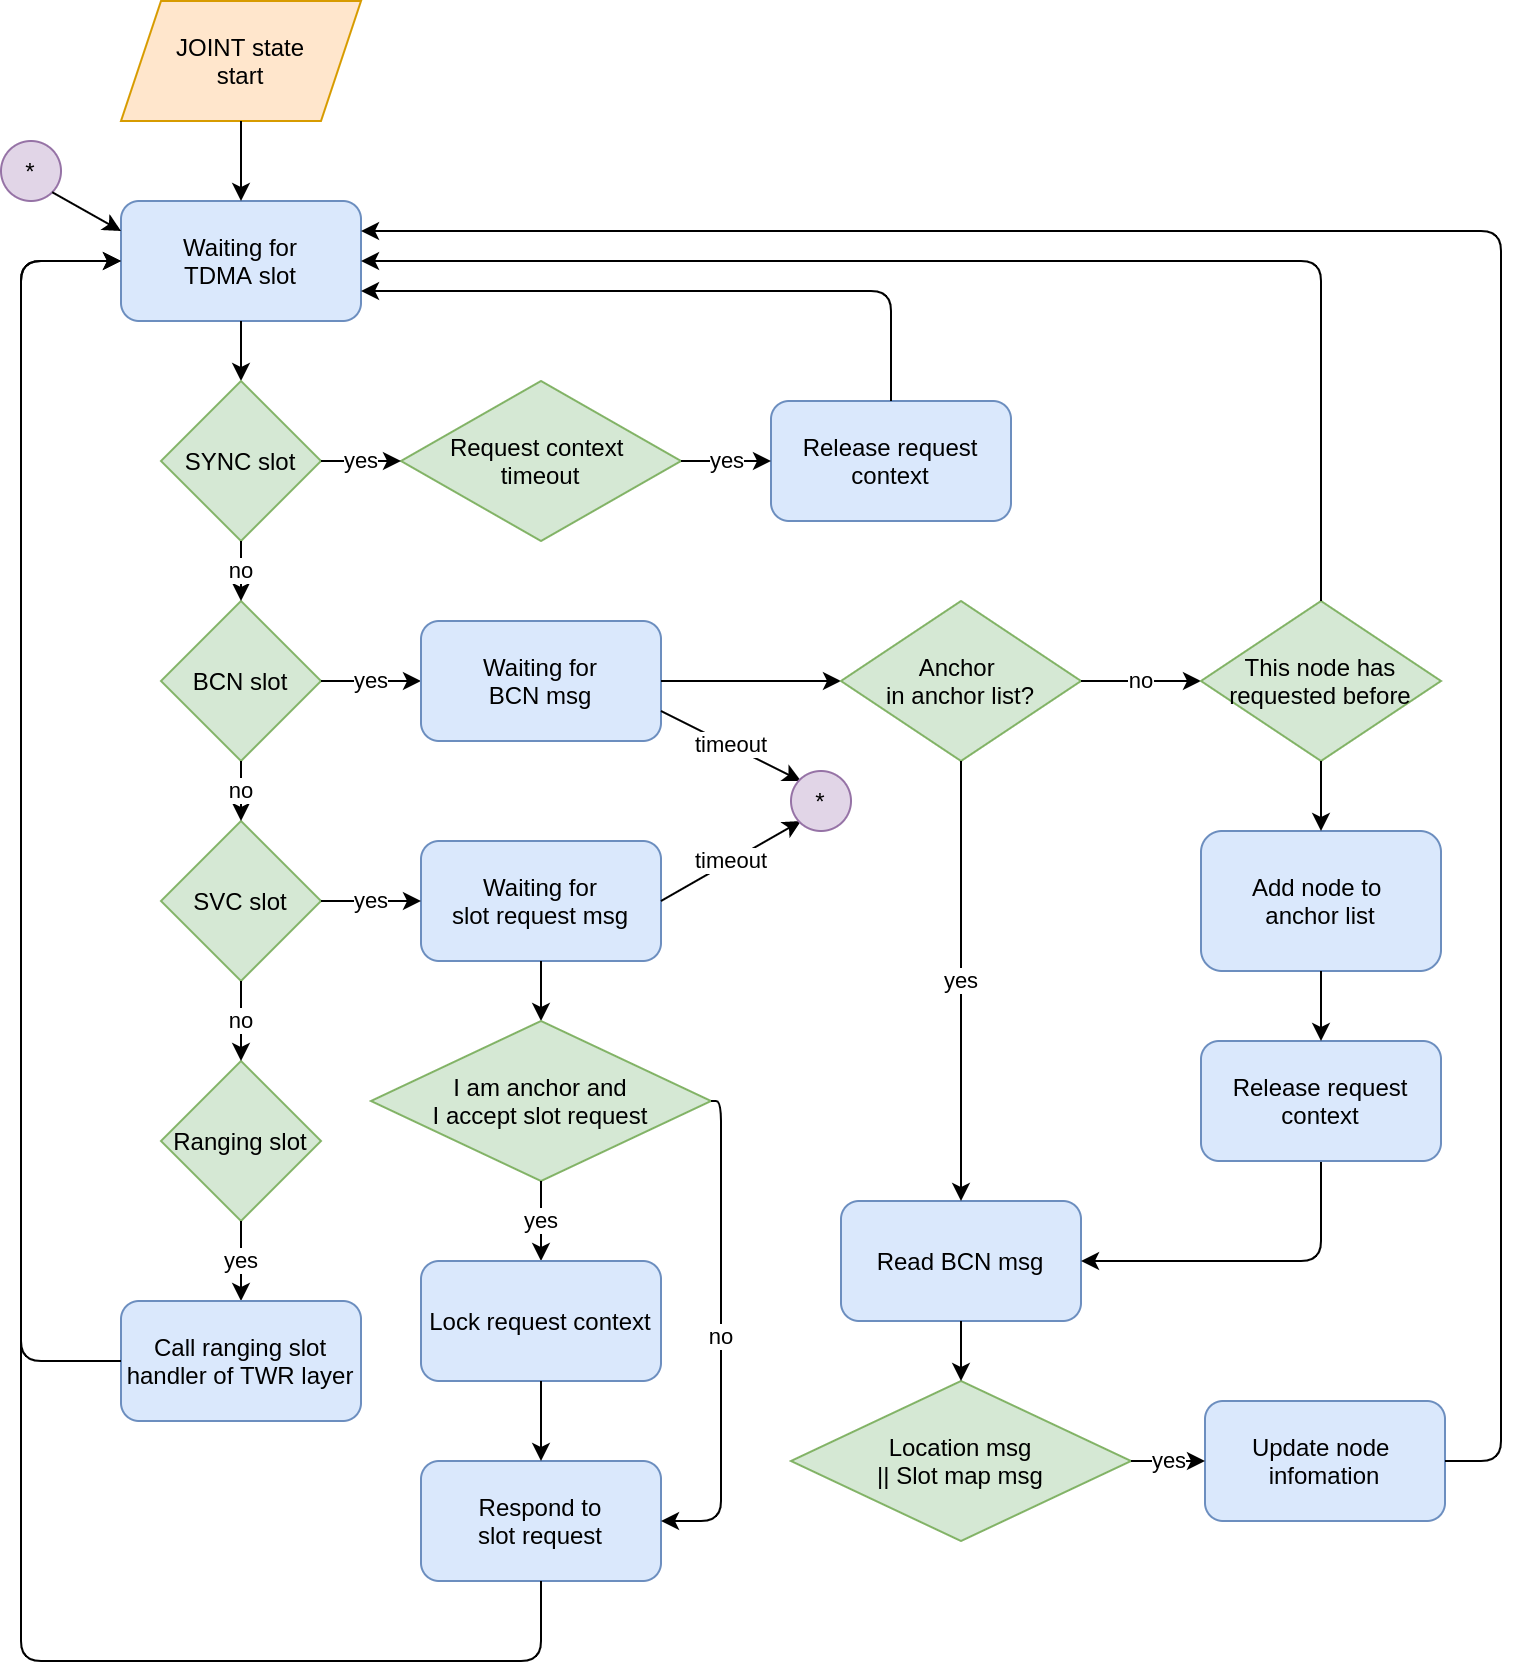
\includegraphics[scale=0.32]{JOINTED_state_flow_chart.png}
    \end{center}
    \caption{JOINTED state diagram}
    \label{fig:JOINTED_state_diagram}
\end{figure}

\section{Two way ranging (TWR)}
By using TWR, the need of synchronized clocks is eliminated since both the round-trip time(s) and the reply time(s) can be calculated separately using timestamps derived from each device.
\begin{figure}[H]
    \begin{center}
        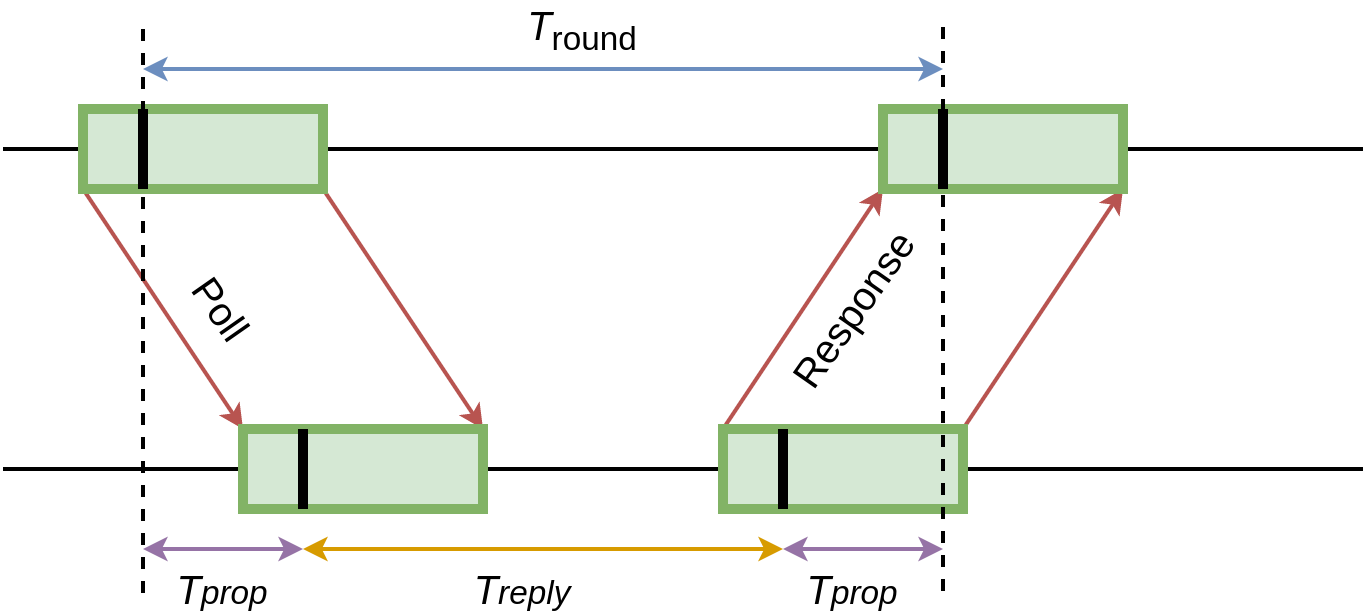
\includegraphics[scale=0.5]{single_sided_two_way_ranging.png}
    \end{center}
    \caption{Single-sided two-way ranging}
    \label{fig:single_sided_two_way_ranging}
\end{figure}

\begin{figure}[H]
    \begin{center}
        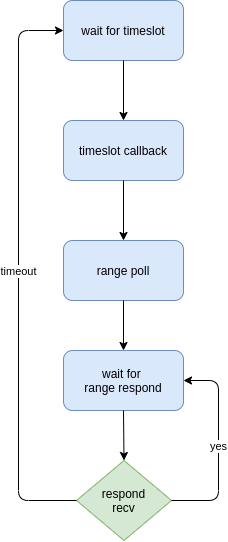
\includegraphics[scale=0.5]{twr_initiator.png}
    \end{center}
    \caption{TWR initiator flow chart}
    \label{fig:twr_initiator}
\end{figure}

\begin{figure}[H]
    \begin{center}
        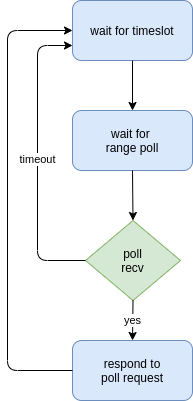
\includegraphics[scale=0.5]{twr_responder.png}
    \end{center}
    \caption{TWR responder flow chart}
    \label{fig:twr_responder}
\end{figure}

\subsection{Wireshark extension for capturing packets}

\bib
\end{document}